\documentclass[11pt,a4paper]{article}

% Packages
\usepackage[utf8]{inputenc}
\usepackage[english]{babel}
\usepackage{caption}
\usepackage{listings}
\usepackage{adjustbox}
\usepackage{enumitem}
\usepackage{dsfont}
\usepackage{boldline}
\usepackage{amssymb, amsmath}
\usepackage[margin=1in]{geometry}
\usepackage{xcolor}
\usepackage{enumerate}
\usepackage{hyperref}
\usepackage{graphics, graphicx, float}
\usepackage{titlesec} %\titleformat

% Meta
\title{Introduction to Multivariate Data Analysis
	\\\medskip \large Final Project Report}
\author{José Antonio Álvarez Ocete - 917933752 \\ jocete@ucdavis.edu}
\date{ \today }

% Custom
\providecommand{\abs}[1]{\lvert#1\rvert}
\setlength\parindent{0pt}
\definecolor{Light}{gray}{.90}
\setlength{\parindent}{1.5em} %sangria

% Thicker lines in tables
\makeatletter
\newcommand{\thickhline}{%
	\noalign {\ifnum 0=`}\fi \hrule height 1pt
	\futurelet \reserved@a \@xhline
}
\makeatother

% Subsubsubsection (|paragraph)
\setcounter{tocdepth}{4}
\setcounter{secnumdepth}{4}

\begin{document}	
	
	\maketitle 
	\newpage
	\tableofcontents
	\newpage
	
	\section{Multiple Linear Regression}
	
	\subsection{Introduction}
	
	In this first section, we will conduct a multiple linear regression following question 1 of the 5th homework assignment. We will estimate the regression coefficients (betas) following different several methods seen during the lectures and we will provide an estimation for a new response.
	
	\subsection{Summary}
	
	For this first analysis, I've selected the Battery Failure dataset. In this example, we want to predict the cycles of life of a certain battery before it fails. We are provided the following variables: Charge rate (amps), discharge rate (amps), depth of discharge (\% of rated ampere-hours), temperature (ºC), and end of charge voltage (volts). These are the first three rows of data: 
	
	\begin{table}[H] \centering
		\begin{tabular}{|cccccc|}
			\hline
			\begin{tabular}[c]{@{}c@{}}Charge rate\\  (amps)\end{tabular} & \begin{tabular}[c]{@{}c@{}}Discharge Rate\\ (amps)\end{tabular} & \begin{tabular}[c]{@{}c@{}}Depth of \\ Discharge\\ (\% of rated\\ ampere-hours)\end{tabular} & \begin{tabular}[c]{@{}c@{}}Temperature\\ (ºC)\end{tabular} & \begin{tabular}[c]{@{}c@{}}End of\\ Charge\\ Voltage\\ (volts)\end{tabular} & \begin{tabular}[c]{@{}c@{}}Cicles to\\ failure\end{tabular} \\ \hline
			0.375                                                         & 3.13                                                            & 60.0                                                                                         & 40                                                         & 2.00                                                                        & 101                                                         \\
			1.000                                                         & 3.13                                                            & 76.8                                                                                         & 30                                                         & 1.99                                                                        & 141                                                         \\
			1.000                                                         & 3.13                                                            & 60.0                                                                                         & 20                                                         & 2.00                                                                        & 96                                                          \\ \hline
		\end{tabular}
	\end{table}
	
	\subsection{Analysis}
	
	\textbf{(1) Find the least square estimate beta hat} \\
	
	We obtain the least square estimate beta hat following out notes:
	
	$$ \hat{\vec{\beta}} = (Z^T \cdot Z)^{-1} \cdot Z^T \cdot \vec{Y} $$
	
	Obtaining:
	$$ \hat{\vec{\beta}} =
		\begin{pmatrix}
		-2937.7571 \\
		-33.7934   \\
		-0.1798   \\
		-1.7397    \\
		7.0627     \\
		1529.2897
		\end{pmatrix}
	$$
	
	\textbf{(2) Find the $R^2$ statistic} \\
	
	We use:
	
	$$ R^2 = \frac{||\hat{\vec{Y}} - \bar{Y} \cdot \vec{1_n}||^2}{||\vec{Y} - \bar{Y} \cdot \vec{1_n}||^2} $$
	
	Obtaining $R^2 = 0.4799$. \\
	
	\textbf{(3) Find sigma\_hat\_square and estimated Cov(beta square)} \\
	
	We use:
	
	$$ \hat{\sigma}^2 = \frac{1}{n-r-1} ||\hat{\vec{\epsilon}}||^2 $$
	
	and
	
	$$ \hat{Cov}(\hat{\vec{\beta}}) = \hat{\sigma}^2 (Z^T Z)^{-1} $$
	
	We obtain the following:
	
	$$ \hat{\sigma}^2 = 7138.186 $$	
	$$ \hat{Cov}(\hat{\vec{\beta}}) = 
	\begin{pmatrix}
	1.633e+07  & -2933.74 & 2980.4460  & -34.78143 & -991.73637 & -8.160e+06 \\
	-2.934e+03 & 1880.55  & 18.5503    & 17.34897  & 10.28445   & -1.764e+02 \\
	2.980e+03  & 18.55    & 193.4117   & -3.23257  & 0.34449    & -1.696e+03 \\
	-3.478e+01 & 17.35    & -3.2326    & 1.79944   & -0.08092   & -4.242e+01 \\
	-9.917e+02 & 10.28    & 0.3445     & -0.08092  & 3.89193    & 4.549e+02  \\
	-8.160e+06 & -176.39  & -1695.7845 & -42.42251 & 454.86652  & 4.081e+06 
	\end{pmatrix}
	$$ \\
	
	\textbf{(4) 95\% confidence interval for each $\beta_j$} \\
	
	We use one at a time confidence intervals for the betas:
	
	$$ \beta_j \in [ \hat{\beta_j} \pm \hat{\sigma} \cdot \sqrt{\omega_{jj}} \cdot t_{n-r-1}(\frac{\alpha}{2}) ] $$
	
	Obtaining:
	
	\begin{table}[H] \centering
		\begin{tabular}{l}
			$\beta_0 \in [ -11604 , 5729 ]$ \\
			$\beta_1 \in [ -126.8 , 59.22 ]$ \\
			$\beta_2 \in [ -30.01 , 29.65 ]$ \\
			$\beta_3 \in [ -4.617 , 1.137 ]$ \\
			$\beta_4 \in [ 2.831 , 11.29 ]$ \\
			$\beta_5 \in [ -2804 , 5862 ]$
		\end{tabular}
	\end{table}
	
	\textbf{(5) 95\% simultaneous confidence intervals for all betas based on the confidence region} \\
	
	Using the formula from the notes:
	
	$$ \beta_j \in [ \hat{\beta_j} \pm \hat{\sigma} \cdot \sqrt{\omega_{jj}} \cdot \sqrt{(r+1) \cdot F_{r+1,n-r-1}(\alpha)} ] $$
	
	We obtain:
	
	\begin{table}[H] \centering
		\begin{tabular}{l}
			$\beta_0 \in [ -19640 , 13764 ]$ \\
			$\beta_1 \in [ -213 , 145.5 ]$ \\
			$\beta_2 \in [ -57.67 , 57.31 ]$ \\
			$\beta_3 \in [ -7.285 , 3.805 ]$ \\
			$\beta_4 \in [ -1.092 , 15.22 ]$ \\
			$\beta_5 \in [ -6822 , 9880 ]$
		\end{tabular}
	\end{table}
	
	\textbf{(6) 95\% simultaneous confidence intervals for all betas based on the Bonferroni correction} \\
	
	We compute a final set of intervals for the ebtas using the Bonferroni correction:
	
	$$ \beta_j \in [ \hat{\beta_j} \pm \hat{\sigma} \cdot \sqrt{\omega_{jj}} \cdot t_{n-r-1}(\frac{\alpha}{2(r+1)}) ] $$
	
	We obtain:
	
	\begin{table}[H] \centering
		\begin{tabular}{l}
			$\beta_0 \in [ -15338 , 9462 ]$ \\
			$\beta_1 \in [ -166.9 , 99.29 ]$ \\
			$\beta_2 \in [ -42.86 , 42.5 ]$ \\
			$\beta_3 \in [ -5.856 , 2.377 ]$ \\
			$\beta_4 \in [ 1.009 , 13.12 ]$ \\
			$\beta_5 \in [ -4670 , 7729 ]$
		\end{tabular}
	\end{table}
	
	\textbf{(7) Test $H_0: \beta_1 = \beta_2 = 0 $ at significance level $\alpha = 0.05$} \\
	
	Using this matrix for the linear transformation:
	
	$$ C = 
	\begin{pmatrix}
		0 & 1 & 0 & 0 & 0 & 0 \\
		0 & 0 & 1 & 0 & 0 & 0 \\
		0 & 0 & 0 & 1 & 0 & 0 \\
		0 & 0 & 0 & 0 & 1 & 0 \\
		0 & 0 & 0 & 0 & 0 & 1
	\end{pmatrix}
	$$
	
	We can compute the F-test statistic:
	
	$$ \vec{\beta}^T_{(2)} \Omega_{22}^{-1} \vec{\beta}_{(2)} = 108296 $$
	
	And compare it to:
	
	$$ (r-q) \cdot \hat{\sigma}^2 \cdot F_{r-q,n-r-1}(\alpha) = 133445 $$
	
	Since $108296 < 133445$, we don't have sufficient evidence to assure that $\beta_1 = \beta_2 = 0$. \\
	
	\textbf{(8) 95\% confidence interval for the mean response given $\mathds{E}(Y_0) = \beta_0 + \sum_{i=1}^{5} \beta_i \cdot \bar{z}_i$, where $\bar{z}_i$ is the sample mean of $z_{i,j}$ for $i \in \{1, ..., n\}$} \\
	
	First, compute $\vec{z_0}$:
	
	$$ \vec{z_0} = 
	\begin{pmatrix}
		1.000  \\
		1.031  \\
		3.034  \\
		62.840 \\
		19.500 \\
		1.999 
	\end{pmatrix} 
	$$
	
	And now compute the confidence intervals for it's associated value using the formula in the class notes:
	
	$$ \vec{z_0}^T \vec{\beta} \in [\vec{z_0}^T \hat{\vec{\beta}} \pm \hat{\sigma} \cdot t_{n-r-1}(\frac{\alpha}{2}) \sqrt{\vec{z_0}^T (Z^T Z)^{-1} \vec{z_0}} ] $$
	
	Obtaining the following interval: $ \vec{z_0}^T \vec{\beta} \in [ 71.78 , 152.8 ] $ \\
	
	\textbf{(9) 95\% confidence interval for a new response $Y_0$ given $\vec{z_0}$} \\
	
	Using a similiar formula: 
	
	$$ \vec{z_0}^T \vec{\beta} \in [\vec{z_0}^T \hat{\vec{\beta}} \pm \hat{\sigma} \cdot t_{n-r-1}(\frac{\alpha}{2}) \sqrt{1 + \vec{z_0}^T (Z^T Z)^{-1} \vec{z_0}} ] $$
	
	And using that $Y_0 = \vec{z_0}^T \vec{\beta} + \epsilon_0$ we obtain:
	
	$$ Y_0 \in [ -73.38 , 298 ] $$
	
	A substantialy bigger interval than the over in \textbf{(8)}, which makes sense since we are including the error now.
	
	\section{Principal Component Analysis}
	
	\subsection{Introduction}
	Briefly summarize the goal of the analysis in your own words
	\subsection{Summary}
	Summarize your data by plots or sample estimates
	\subsection{Analysis}
	Implement the analysis based on what you have done in homework
	
	
	\section{Two-Sample test and Linear Discriminant Analysis}
	
	\subsection{Introduction}
	
	For this final analysis we will conduct Linear Discriminant Analysis. That is, given enough data about tagged as two different classes, classify a new reponse into one of this classes. In order to do that we first need to conduct a two sample test to make sure that our populations are actually different.
	
	\subsection{Summary}
	
	The dataset selection for this example was a little trickier since I wanted to display nice graphs about the data. In order to achieve this the more convinient way was to pick up a two-variate dataset with a nice visual separation between its classes. We will see why in the analysis. \\
	
	The dataset selected was the Anaconda one. It has two variates: Snout vent length and weight. The class we want to predict is the snake gender: either male (M) or female (F). These are the first 5 rows of our dataset from each class:
	
	\begin{table}[H] \centering
		\begin{tabular}{|ccc|ccc|}
			\hline
			Snout Vent Length & Weight & Gender & Snout Vent Length & Weight & Gender \\ \hline
			271.0             & 18.50  & F      & 176.7             & 3.00   & M      \\
			477.0             & 82.50  & F      & 259.5             & 9.75   & M      \\
			306.3             & 23.40  & F      & 258.0             & 10.07  & M      \\
			365.3             & 33.50  & F      & 229.8             & 7.50   & M      \\
			466.0             & 69.00  & F      & 233.0             & 6.25   & M      \\
			440.7             & 54.00  & F      & 237.5             & 9.85   & M      \\ \hline
		\end{tabular}
	\end{table}
	
	Our dataset is completely balanced, having the same number of males than females.
	
	\subsection{Analysis}
	
	As stated in the introduction we start by conduction a two sample test with the null hypothesis $H_0: \mu_1 = \mu_2$. We start by extracting the basic stats from the data and computing the Hotelling's $T^2$ statistic:
	
	$$ \bar{\vec{x_1}} = 
	\begin{pmatrix}
	348.28  \\         
	37.26
	\end{pmatrix} 
	, \bar{\vec{x_2}} = 
	\begin{pmatrix}
	228.75  \\         
	7.29
	\end{pmatrix} 
	$$
	
	$$ S_{pooled} = 
	\begin{pmatrix}
		\multicolumn{1}{c}{2606.4} & \multicolumn{1}{c}{667.9} \\
		667.9                      & 204.2                    
	\end{pmatrix} 
	$$ 
	
	$$ T^2 = (\bar{\vec{x_1}} - \bar{\vec{x_2}})^T ((\frac{1}{n_1} + \frac{1}{n_2}) S_{pooled})^{-1} (\bar{\vec{x_1}} - \bar{\vec{x_2}}) = 76.92 $$ 
	
	We compare this value to:
	
	$$ F = \frac{(n_1 + n_2 - 2)p}{n_1+n_2-1-p} \cdot F_{p, n_1+n_2-1-p}(\alpha) = 6.463 $$
	
	Since $76.92 > 6.463$, we reject $H_0$, concluding that both population are, indeed, different. We can now procede with linear discrimination analysis. For a given new response $\vec{x_0}$ we will classify it in the first population if and only if:
	
	$$ (\bar{\vec{x_1}} - \bar{\vec{x_2}})^T \cdot S_{pooled}^{-1} \cdot (\vec{x_0} - \frac{1}{2}(\bar{\vec{x_1}} - \bar{\vec{x_2}})) \ge 0 $$
	
	That is, if and only if:
	
	$$ 0.05095 - 0.01986 \cdot (\vec{x_0} - \begin{pmatrix}
	288.5 \\
	22.28
	\end{pmatrix} ) \ge 0 $$
	
	In order to meassure how good this classifier is we use two methods:
	
	\begin{itemize}
		\item The Apparent Error Rate (AER): Try to predict every single sample by training the model with every point in the dataset (including the one we will predict), and the use it for the prediction.
		\item The Expected Actual Error Rate (EAER): Using the same tachnique but exclude the point that we will predict from the train set.
	\end{itemize}

	In this case we obtain the same value for both measures: a $0.08929 = \frac{5}{56}$ error rate, missing 5 samples. Finally, let's plot our populations and their respective mean-cenetered mahalanobis-distance elipses:
	
	\begin{figure}[H] 
		\centering
		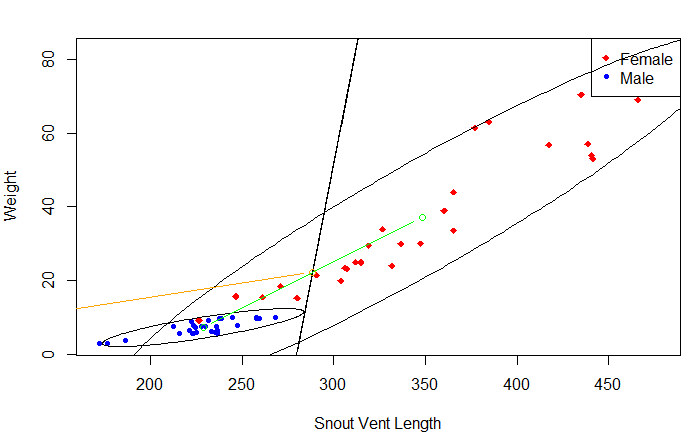
\includegraphics[scale=.9]{./pics/LDA}
		%\caption{my-captino} \label{my-label}
	\end{figure}
	
	
\end{document}